\documentclass{article}\usepackage[]{graphicx}\usepackage[]{xcolor}
% maxwidth is the original width if it is less than linewidth
% otherwise use linewidth (to make sure the graphics do not exceed the margin)
\makeatletter
\def\maxwidth{ %
  \ifdim\Gin@nat@width>\linewidth
    \linewidth
  \else
    \Gin@nat@width
  \fi
}
\makeatother

\definecolor{fgcolor}{rgb}{0.345, 0.345, 0.345}
\newcommand{\hlnum}[1]{\textcolor[rgb]{0.686,0.059,0.569}{#1}}%
\newcommand{\hlsng}[1]{\textcolor[rgb]{0.192,0.494,0.8}{#1}}%
\newcommand{\hlcom}[1]{\textcolor[rgb]{0.678,0.584,0.686}{\textit{#1}}}%
\newcommand{\hlopt}[1]{\textcolor[rgb]{0,0,0}{#1}}%
\newcommand{\hldef}[1]{\textcolor[rgb]{0.345,0.345,0.345}{#1}}%
\newcommand{\hlkwa}[1]{\textcolor[rgb]{0.161,0.373,0.58}{\textbf{#1}}}%
\newcommand{\hlkwb}[1]{\textcolor[rgb]{0.69,0.353,0.396}{#1}}%
\newcommand{\hlkwc}[1]{\textcolor[rgb]{0.333,0.667,0.333}{#1}}%
\newcommand{\hlkwd}[1]{\textcolor[rgb]{0.737,0.353,0.396}{\textbf{#1}}}%
\let\hlipl\hlkwb

\usepackage{framed}
\makeatletter
\newenvironment{kframe}{%
 \def\at@end@of@kframe{}%
 \ifinner\ifhmode%
  \def\at@end@of@kframe{\end{minipage}}%
  \begin{minipage}{\columnwidth}%
 \fi\fi%
 \def\FrameCommand##1{\hskip\@totalleftmargin \hskip-\fboxsep
 \colorbox{shadecolor}{##1}\hskip-\fboxsep
     % There is no \\@totalrightmargin, so:
     \hskip-\linewidth \hskip-\@totalleftmargin \hskip\columnwidth}%
 \MakeFramed {\advance\hsize-\width
   \@totalleftmargin\z@ \linewidth\hsize
   \@setminipage}}%
 {\par\unskip\endMakeFramed%
 \at@end@of@kframe}
\makeatother

\definecolor{shadecolor}{rgb}{.97, .97, .97}
\definecolor{messagecolor}{rgb}{0, 0, 0}
\definecolor{warningcolor}{rgb}{1, 0, 1}
\definecolor{errorcolor}{rgb}{1, 0, 0}
\newenvironment{knitrout}{}{} % an empty environment to be redefined in TeX

\usepackage{alltt}
\usepackage{amsmath} %This allows me to use the align functionality.
                     %If you find yourself trying to replicate
                     %something you found online, ensure you're
                     %loading the necessary packages!
\usepackage{amsfonts}%Math font
\usepackage{graphicx}%For including graphics
\usepackage{hyperref}%For Hyperlinks
\usepackage[shortlabels]{enumitem}% For enumerated lists with labels specified
                                  % We had to run tlmgr_install("enumitem") in R
\hypersetup{colorlinks = true,citecolor=black} %set citations to have black (not green) color
\usepackage{natbib}        %For the bibliography
\setlength{\bibsep}{0pt plus 0.3ex}
\bibliographystyle{apalike}%For the bibliography
\usepackage[margin=0.50in]{geometry}
\usepackage{float}
\usepackage{multicol}

%fix for figures
\usepackage{caption}
\newenvironment{Figure}
  {\par\medskip\noindent\minipage{\linewidth}}
  {\endminipage\par\medskip}
\IfFileExists{upquote.sty}{\usepackage{upquote}}{}
\begin{document}

\vspace{-1in}
\title{Labs 7 and 8 -- MATH 240 -- Computational Statistics}

\author{
  Pierce Leclerc \\
  Colgate University  \\
  Department of Mathematics  \\
  {\tt pleclerc@colgate.edu}
}

\date{}

\maketitle

\begin{multicols}{2}
\begin{abstract}
In labs 7 and 8, we explored the beta distribution and its properties. We compared summary values of beta distributions under different parameter sets, also analyzing cumulative statistics. We then took death rate data and utilized both the method of moments and maximum likelihood estimates to determine approximate values of the parameters that would provide a matching distribution.
\end{abstract}

\noindent \textbf{Keywords:} Beta Distributions, Random Sampling, Estimators 

\section{Introduction}
The beta distribution is a continuous probability distribution with two free parameters, $\alpha$ and $\beta$. It models a random variable $X$ with a support of $[0,1]$. The parameters can be adjusted to allow for flexibility in the distribution. For example, under specific values of $\alpha$ and $\beta$, a beta distribution can be skewed in different directions, have different excess kurtosis values, and other properties.

\section{Density Functions and Parameters}

Adjusting the parameters of beta distributions, $\alpha$ and $\beta$, can drastically alter their visual properties. Figure 1 provides four examples of different beta distributions.

\begin{Figure}
\begin{center}
  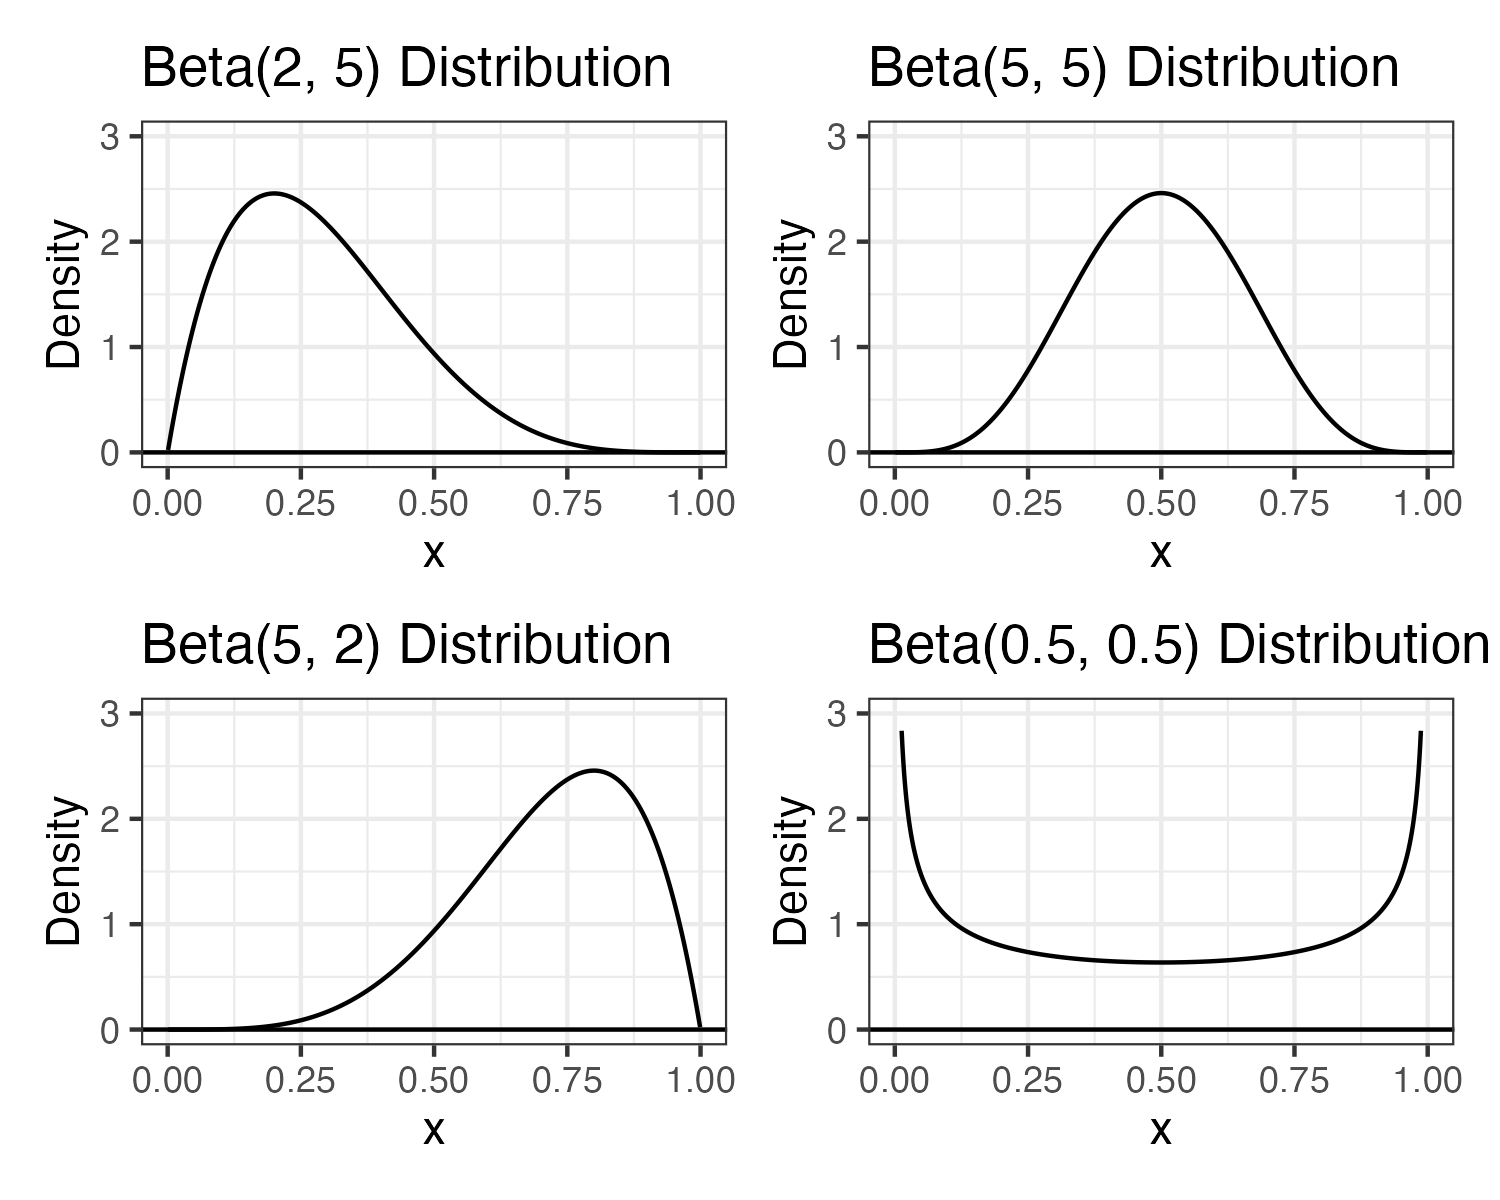
\includegraphics[width=0.5\textwidth]{task1.png}
\end{center}
\captionof{figure}{Beta distributions with different values of $\alpha$ and $\beta$.}
\end{Figure}

From these same four distributions, we can analyze their properties numerically through summaries. Table 1 highlights the mean, variance, skewness, and excess kurtosis of their respective distributions.

\begin{Figure}
\centering
\scriptsize
\begin{tabular}{rrrrrr}
  \hline
 Alpha & Beta & Mean & Variance & Skewness & Excess Kurtosis \\ 
  \hline
2.00 & 5.00 & 0.29 & 0.03 & 0.60 & -0.12 \\ 
5.00 & 5.00 & 0.50 & 0.02 & 0.00 & -0.46 \\ 
5.00 & 2.00 & 0.71 & 0.03 & -0.60 & -0.12 \\ 
0.50 & 0.50 & 0.50 & 0.12 & 0.00 & -1.50 \\ 
   \hline
\end{tabular}
\captionof{table}{Summary values of beta distributions from different choices of $\alpha$ and $\beta$.}
\end{Figure}

From generating samples of each distribution, we can observe how randomly generated data can approximate specific beta distributions in real-world scenarios. Figure 2 illustrates random sampling of the previous beta distributions with both estimated densities and true population densities superimposed.

\begin{Figure}
\begin{center}
  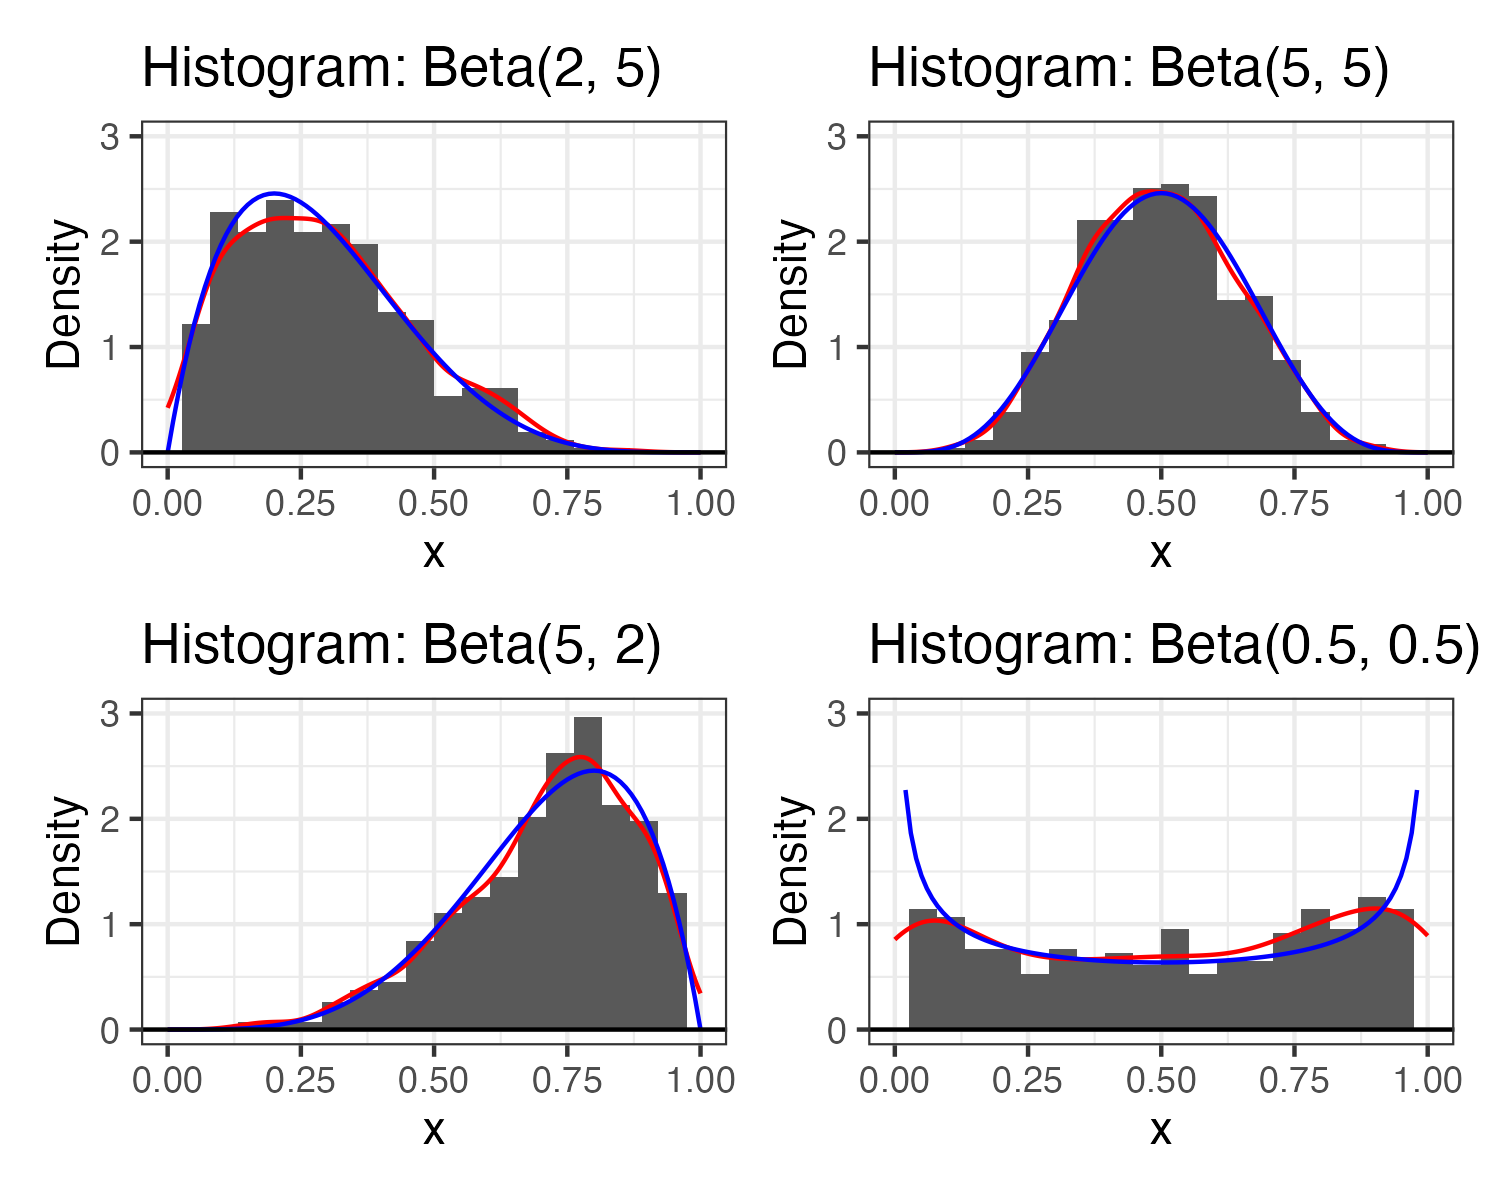
\includegraphics[width=0.5\textwidth]{task3.png}
\end{center} 
\captionof{figure}{Histograms of random samples from different beta distributions.}
\end{Figure}

\section{Properties}

From calculating cumulative statistics, we can attempt to observe convergence to true population quantities as the sample size increases through gradual decreases in variability. Figure 3 demonstrates this convergence through cumulative statistics of sampled data from the Beta(2,5) distribution. As sample size increases, for all four measures, the cumulative statistics visually converge to the values that describe the true population distribution (red horizontal lines).

\begin{Figure}
\begin{center}
  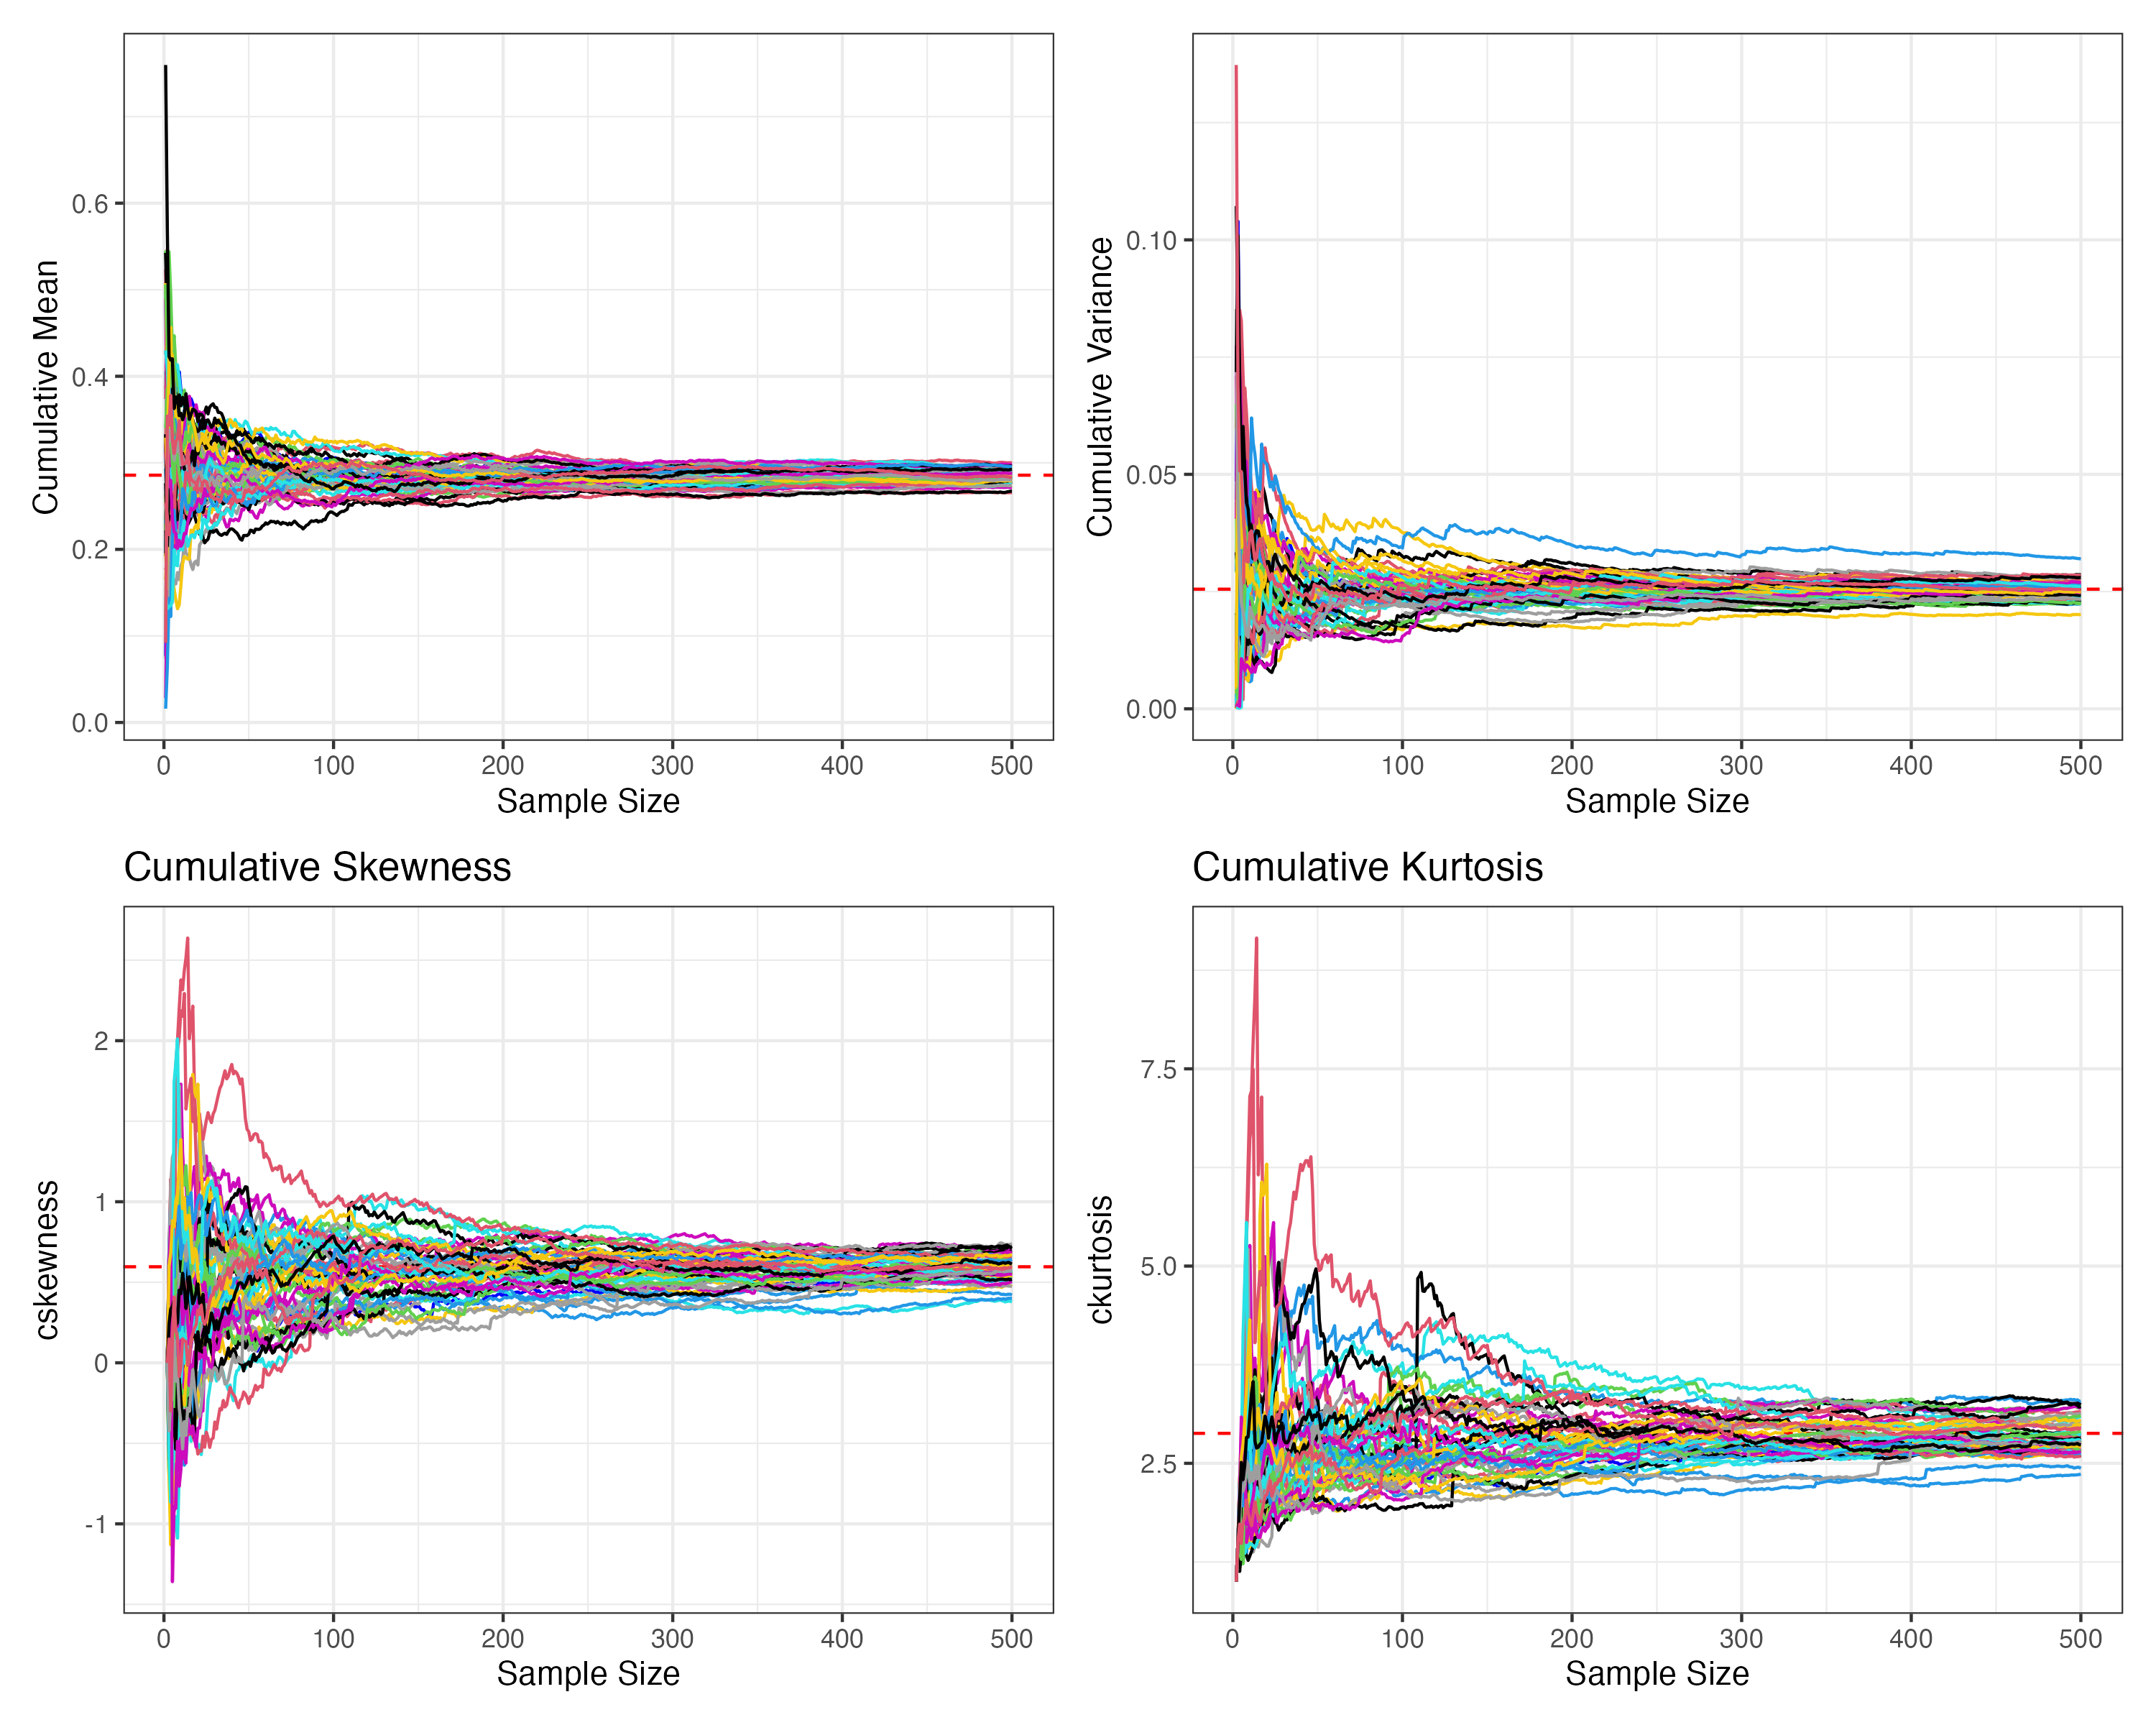
\includegraphics[width=0.5\textwidth]{task4.png}
\end{center} 
\captionof{figure}{Cumulative statistics from sampled data of the Beta(2,5) distribution compared with sample size.}
\end{Figure}

By storing statistics of interest from samples of the Beta(2,5) distribution, we can also observe their likely true values. Figure 4 displays the results, with each statistic appearing normally distributed after 1000 samples were taken.

\begin{Figure}
\begin{center}
  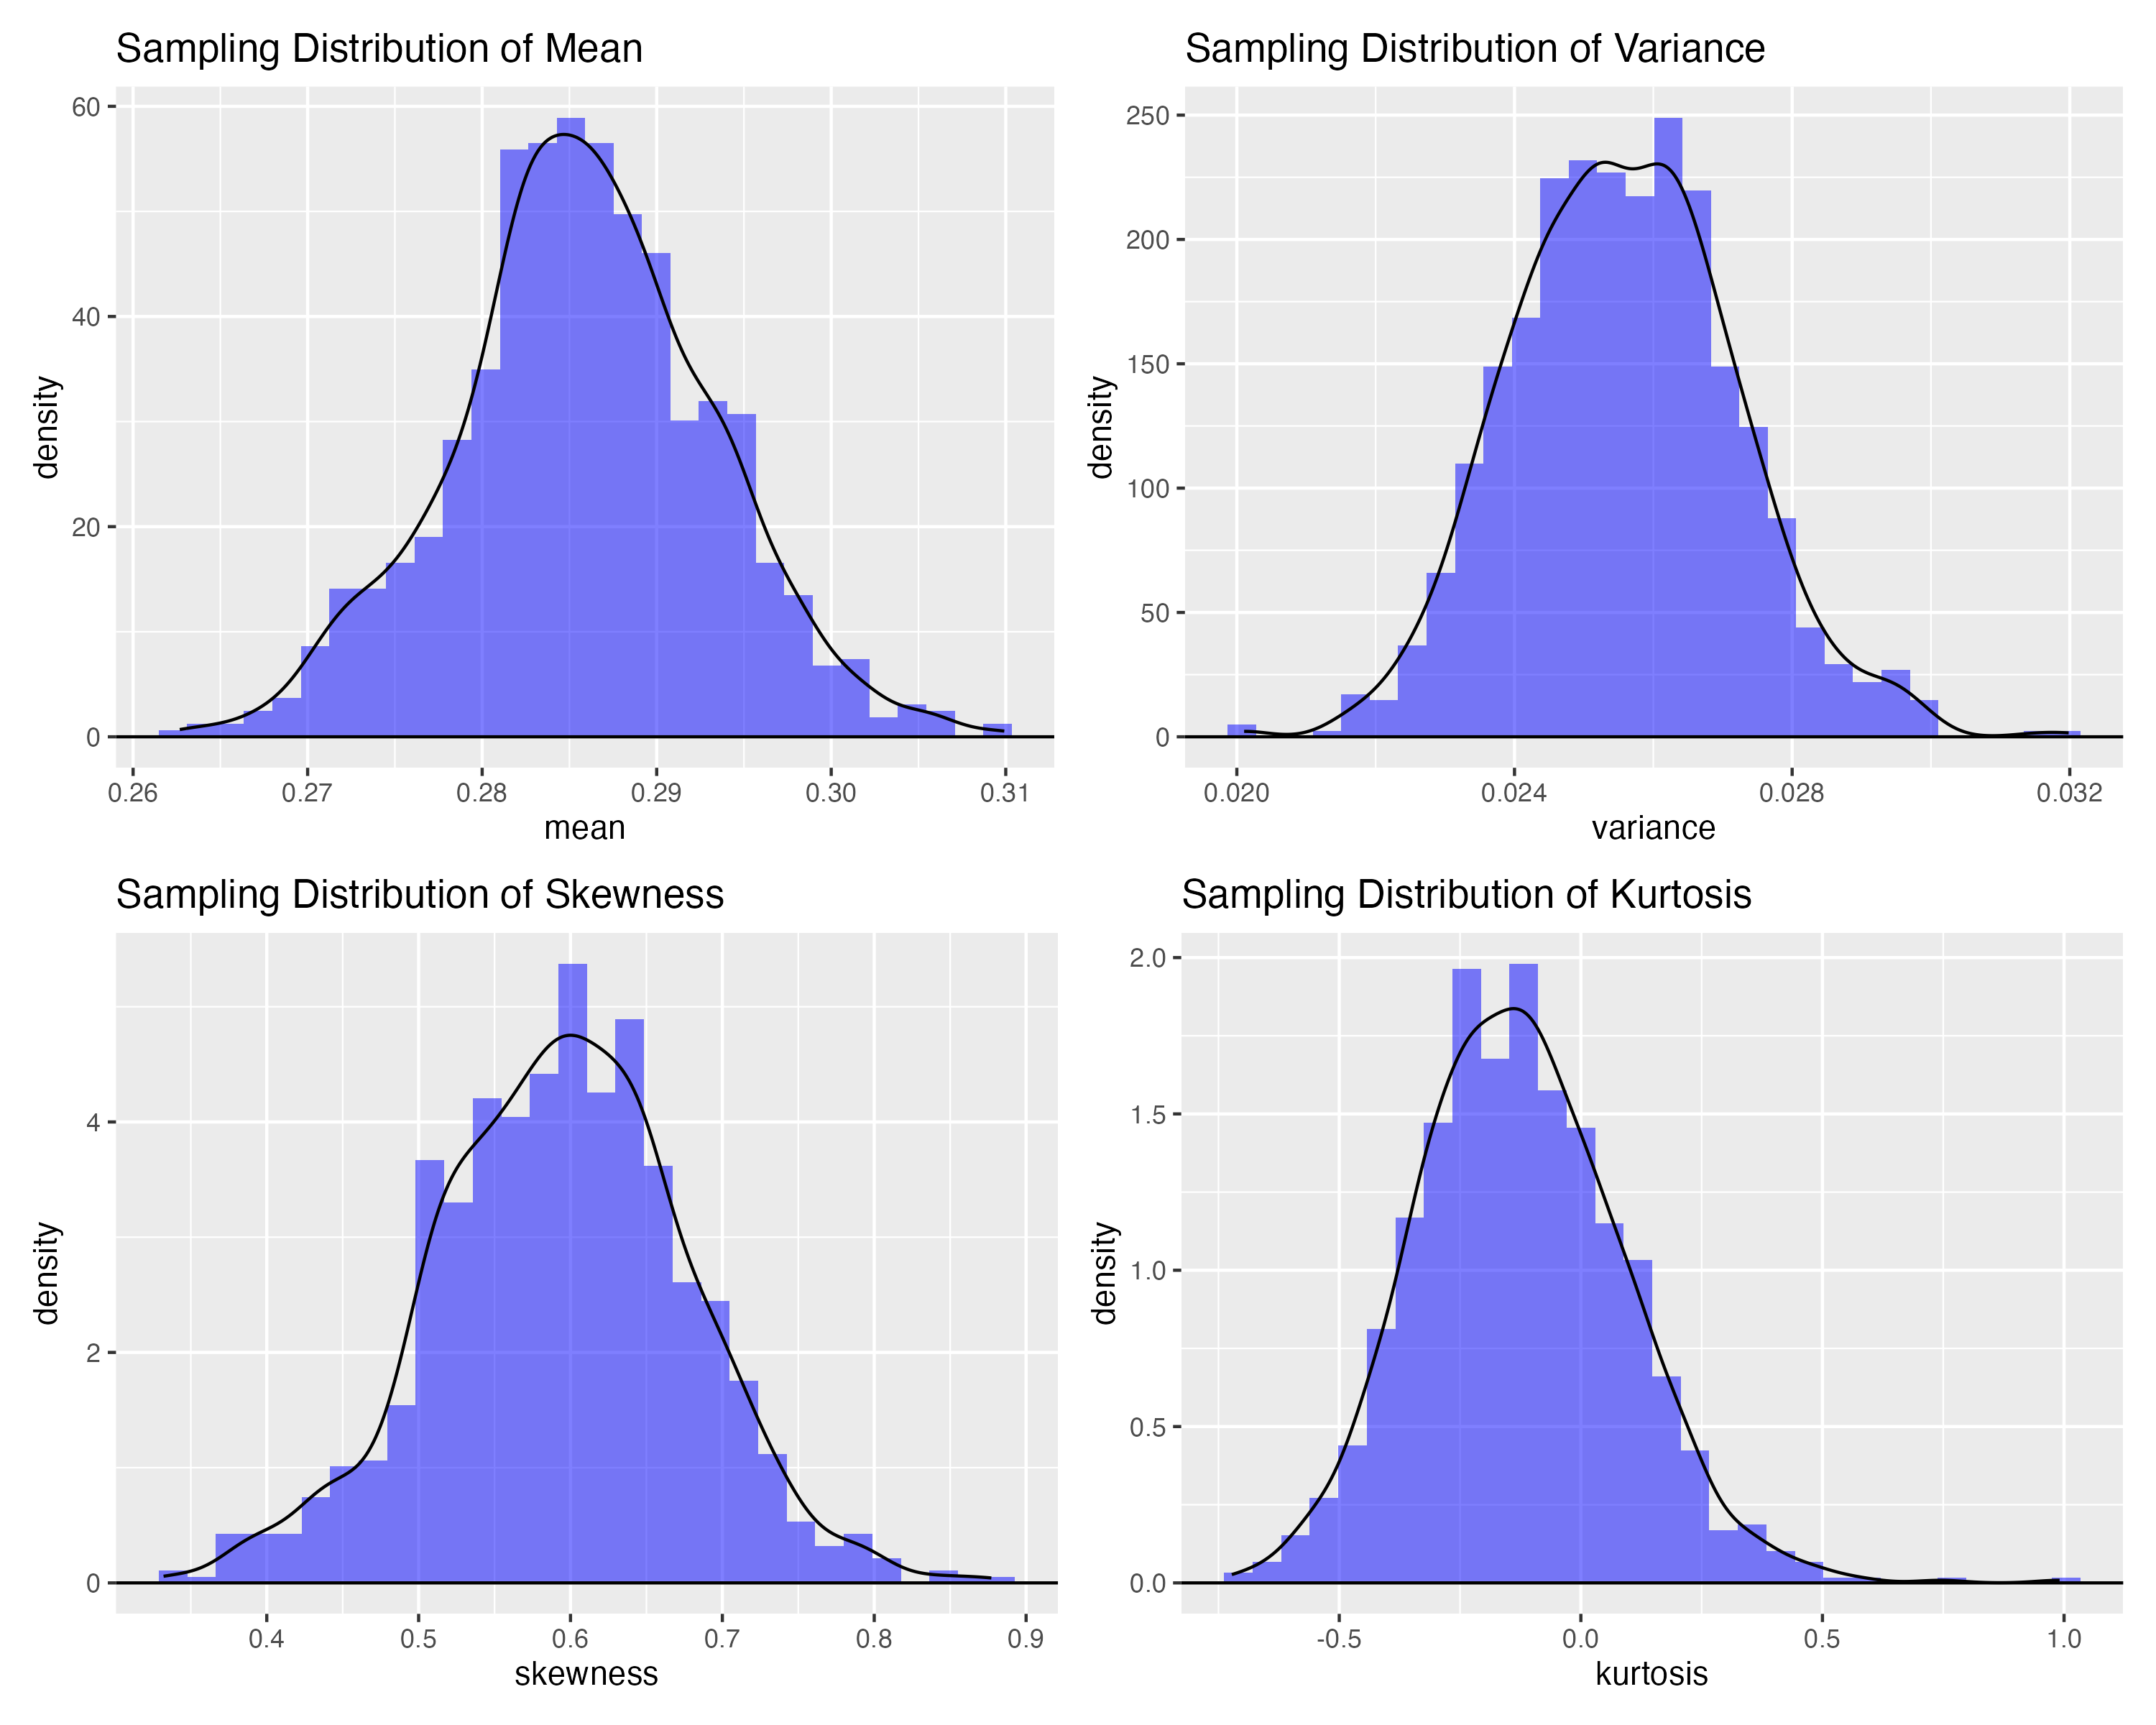
\includegraphics[width=0.5\textwidth]{task5.png}
\end{center} 
\captionof{figure}{Distributions of summary values under random sampling of the Beta(2,5) distribution. All four appear to be normally distributed.}
\end{Figure}

\section{Estimators}

2022 death rate data was collected from the World Bank and analyzed through point estimates in an attempt to determine a beta distribution which the data closely approximates as suggested by \cite{fatih}. Method of moments and maximum likelihood estimators were obtained, and their distributions were superimposed with the death rate data in Figure 5.

\begin{Figure}
\begin{center}
  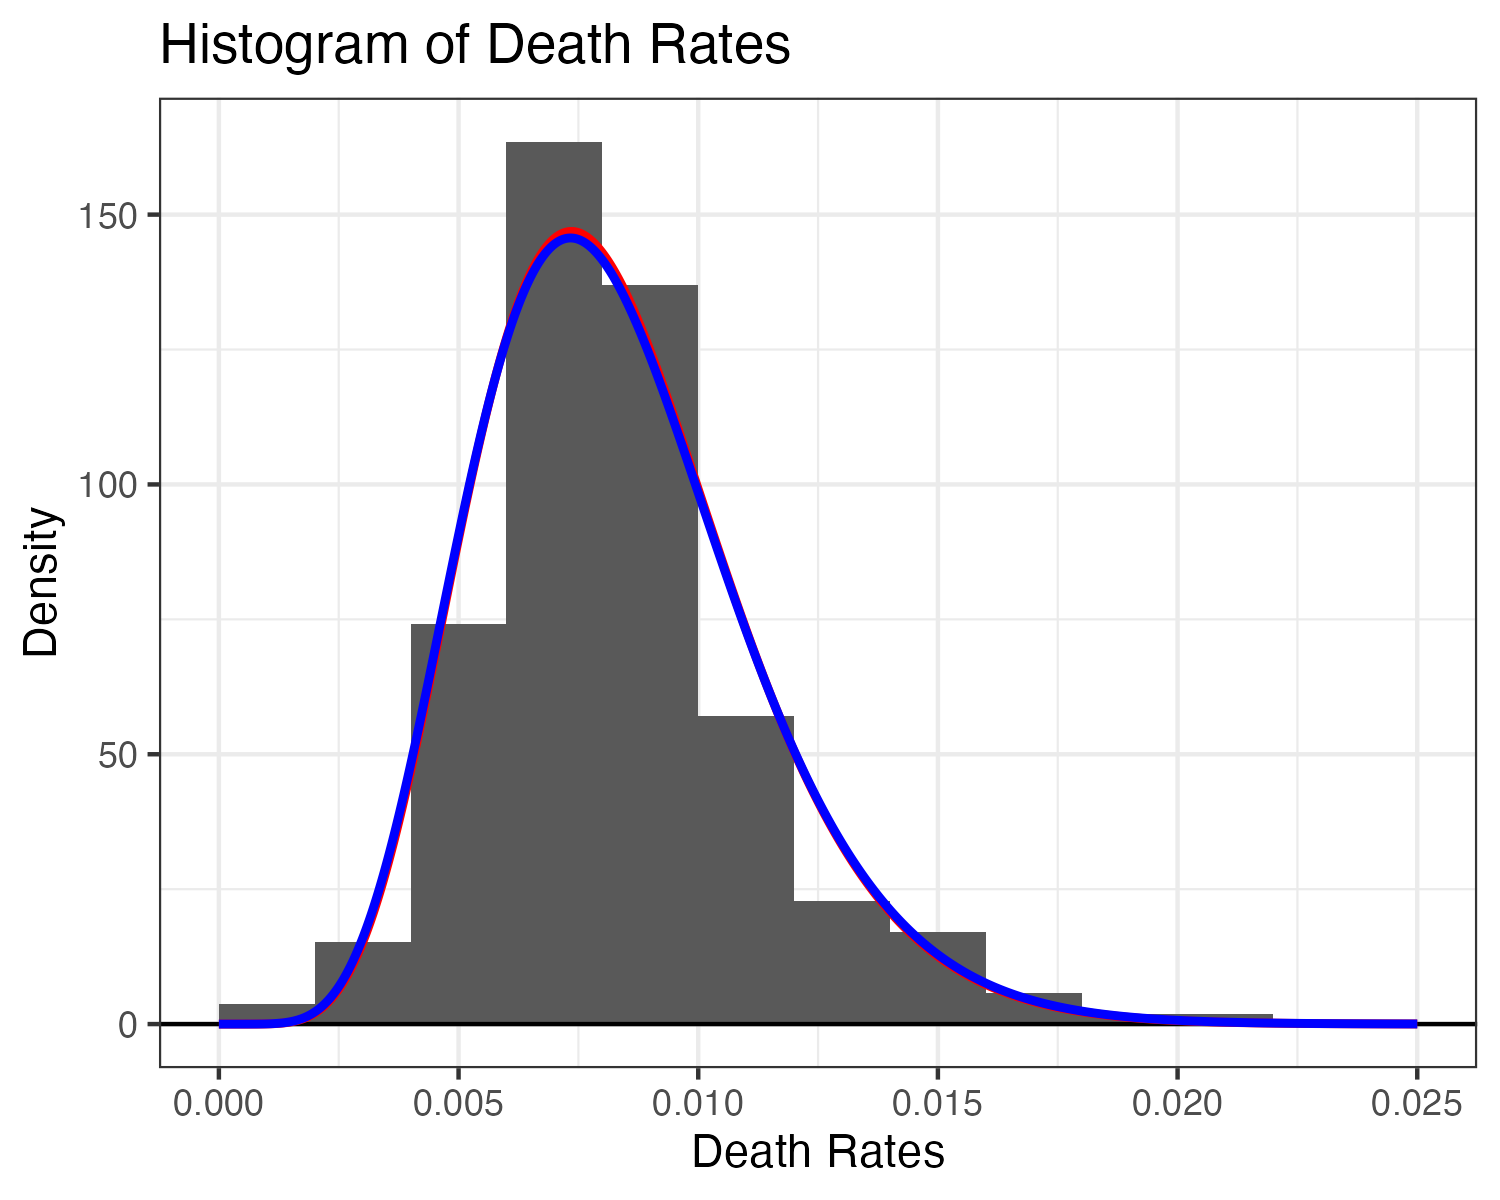
\includegraphics[width=0.5\textwidth]{task7.png}
\end{center} 
\captionof{figure}{Histogram of 2022 death rates from the world bank, with MLE and MoM estimated distributions superimposed.}
\end{Figure}

From 1000 samples, method of moments and maximum likelihood estimators were calculated, and Figure 6 visualizes the densities of each method's respective estimators in an attempt to determine which method provided the best estimates. 

\begin{Figure}
\begin{center}
  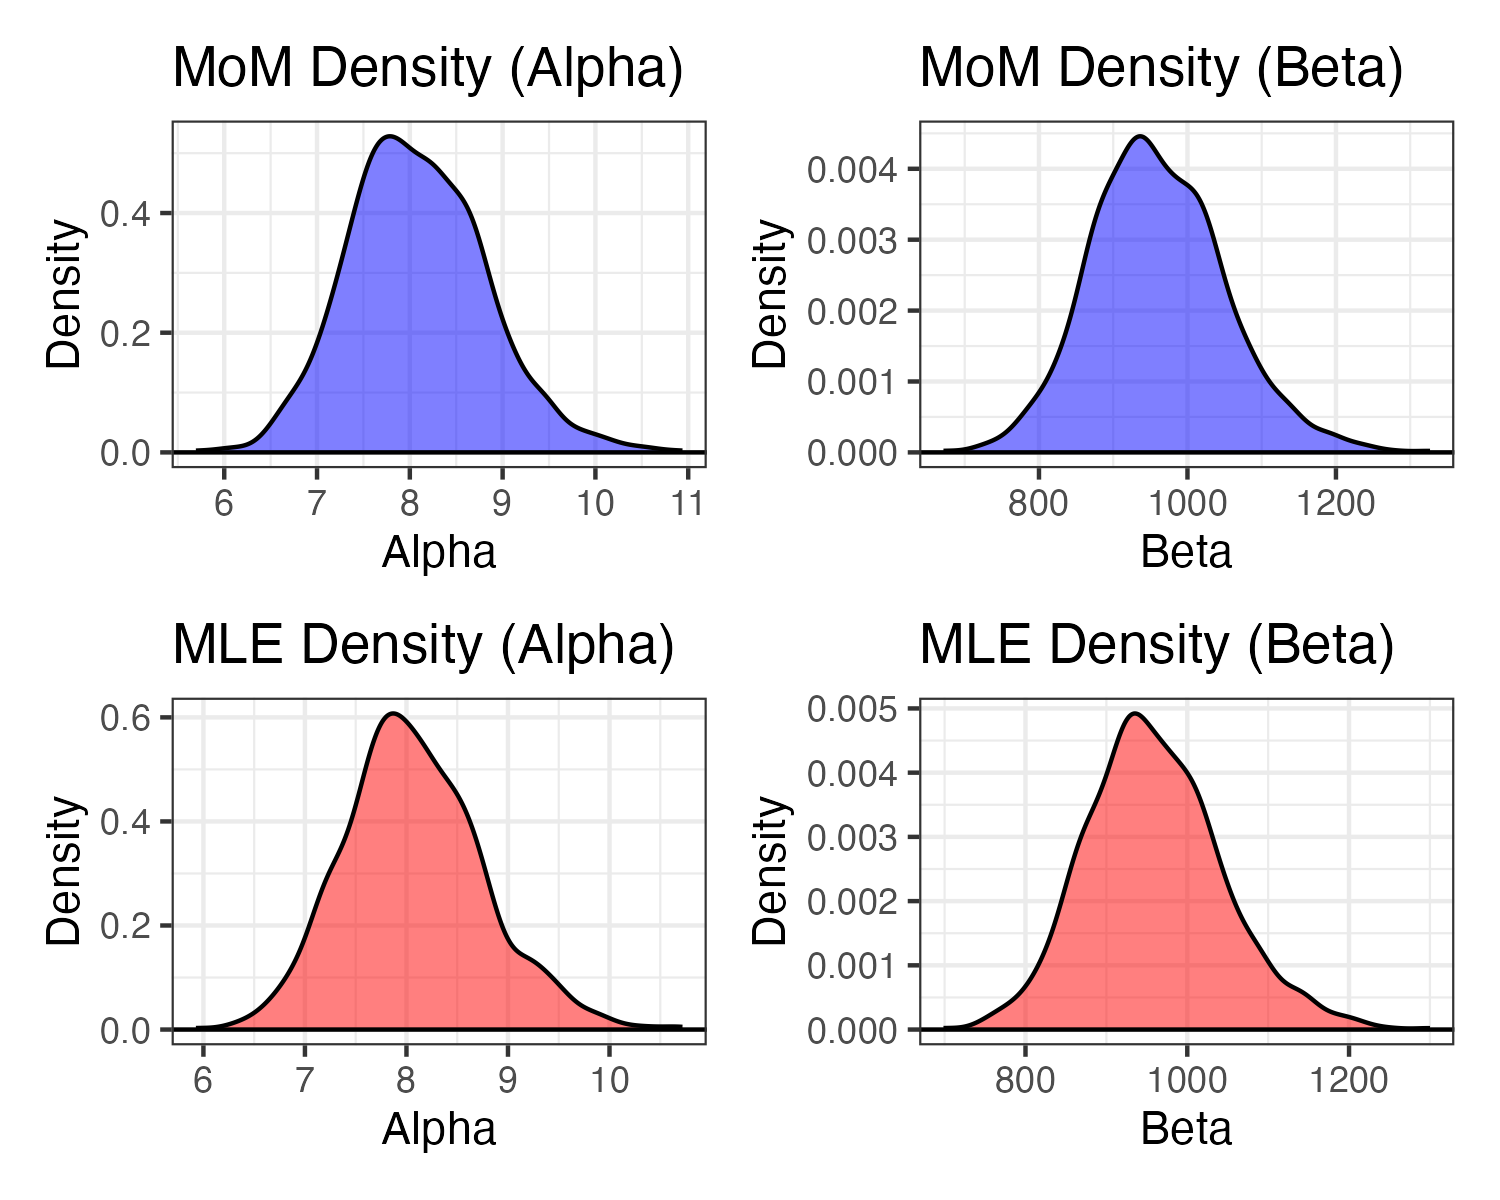
\includegraphics[width=0.5\textwidth]{task8.png}
\end{center} 
\captionof{figure}{Estimated densities of alpha and beta for the method of moments and maximum likelihood estimates.}
\end{Figure}

To aid these visualizations, Table 2 provides a numerical summary, highlighting bias, precision, and mean squared error (MSE) for the estimators.

\begin{Figure}
\centering
\begin{tabular}{llrrr}
  \hline
 Parameter & Method & Bias & Precision & MSE \\ 
  \hline
  Alpha & MoM & 0.08 & 1.83 & 0.55 \\ 
  Alpha & MLE & 0.07 & 2.13 & 0.48 \\ 
  Beta & MoM & 10.29 & 0.00 & 8288.46 \\ 
  Beta & MLE & 9.11 & 0.00 & 7132.70 \\ 
   \hline
\end{tabular}
\captionof{table}{Bias, precision, and mean squared error for the method of moments and maximum likelihood estimates, with $\alpha = 8$ and $\beta = 950$.}
\end{Figure}

From Figure 6 and Table 2, it is evident that the MLE estimators more closely approximate the data, as both bias and MSE are lower for each estimator than their method of moments counterparts.

%%%%%%%%%%%%%%%%%%%%%%%%%%%%%%%%%%%%%%%%%%%%%%%%%%%%%%%%%%%%%%%%%%%%%%%%%%%%%%%%
% Bibliography
%%%%%%%%%%%%%%%%%%%%%%%%%%%%%%%%%%%%%%%%%%%%%%%%%%%%%%%%%%%%%%%%%%%%%%%%%%%%%%%%
\vspace{2em}

\begin{tiny}
\bibliography{bib}
\end{tiny}

\end{multicols}

\end{document}
